\documentclass[]{final_report}
\usepackage{graphicx}
\usepackage{hyperref}
\usepackage{caption}
\usepackage{multirow}
\usepackage{float}
\newfloat{program}{thp}{lop}
\floatname{program}{Code snippet}
%\usepackage[backend=bibtex]{biblatex}
%\bibliography{report_template.bib}
\setcounter{tocdepth}{2}

%%%%%%%%%%%%%%%%%%%%%%
%%% Input project details
\def\studentname{John Patrick Bracken (09442961)}
\def\projecttitle{Reputation Algorithms for the Social Web}
\def\supervisorname{Dr. Michael O'Mahony}
%\def\moderatorname{}
\def\stack{Stack Exchange}


\begin{document}

\maketitle

\begin{specification}

\textbf{\textsl{Subject:}} Social Network Analysis, Reputation Systems

\textbf{\textsl{Coverage}} Social Network Analysis, Reputation Systems

\textbf{\textsl{Project Type:}} Design and Implementation

\textbf{\textsl{Software Requirements:}} Java, Linux, MySQL (or other)

\textbf{\textsl{Hardware Requirements:}} Laptop for development. Access to server will be provided if necessary.

\textbf{\textsl{Preassigned:}} No


\textbf{General Information}

The social web reflects an important paradigm shift in the nature of our online transactions. We increasingly rely on the opinions of others to mediate these transactions and as such the reliability of these users becomes an important indicator of quality. Thus, the concept of user reputation has become increasingly important in the context of today's social web. Recently, there has been considerable research on various approaches to model the reputation of users as they participate in a diverse array of online interactions.

The goal of this project is to design, implement and evaluate reputation algorithms for users of the Stack Exchange network, a popular group of social Q\&A sites. There are currently over 80 topical Stack Exchange websites, hosting almost 2 million users. Some 3.8 million questions have been posed, eliciting 7.7 million answers. Users are permitted to post questions that can be answered by other users in the community. Each answer given can be voted up or down by others and the questioner can chose to highlight a single answer as correct, indicating the question has been answered satisfactorily or that answer was the best answer provided. The availability of such data can be leveraged to estimate the reputation of users; for example, if the answers provided by a particular user are frequently deemed to be correct and/or receive many positive votes from the community, then this provides an indication that the user is knowledgeable about particular subject matters.

\textbf{Mandatory:}
\begin{itemize}
\item Download Stack Exchange data (http://data.stackexchange.com/) - data from three sites should be obtained.
\item Implementation of reputation algorithms from the literature.
\item Evaluation: for each dataset, compare the performance of these algorithms to the user reputation model currently used on Stack Exchange.
\end{itemize}

\textbf{Discretionary:}
\begin{itemize}
\item Predict the correct answers to questions based on user reputation.
\item Evaluate the accuracy of predicted answers.
\item Perform user-trials and correlate prediction performance with offline metrics.
\end{itemize}

\textbf{Exceptional:}

Any (but not limited to) the following:

\begin{itemize}
\item Propose and implement enhancements to improve algorithm performance.
\item Analyse the robustness of the reputation algorithms against attack.
\end{itemize}

\textbf{Reading:}
\begin{itemize}
\item Stack Exchange: http://stackexchange.com/
\item Stack Exchange Data Explorer: http://data.stackexchange.com/
\item A Model of Collaboration-based Reputation for the Social Web – ICWSM 2013 
\item Trust Among Strangers in Internet Transactions: Empirical Analysis of eBay’s Reputation System - Advances in Applied Microeconomics 2012 (attached)
\end{itemize}
\end{specification}

%%%%%%%%%%%%%%%%%%%%%%
%%% Your Abstract herebstract

\begin{abstract}

In this project I intend to compare the performance of generic reputation algorithms using the Stack Exchange Question and Answer sites' open-sourced data dumps. These algorithms will include a simple inbound weighted sum, Page and Brin's PageRank, and Kleinburg's Hubs and Authorities algorithm. Performance will be analysed by evaluating correlation between these algorithms' scores and the bespoke Stack Exchange reputation model.

%I will also attempt to predict the correct answers to questions using user reputation scores, and perform user trials on Q\&A data.

\end{abstract}
\newpage

\chapter*{Acknowledgements}

My thanks go out to my project supervisor Dr. Michael P. O'Mahony  for his help and guidance throughout the course of this project. His kind support epitomises the nature of a good educator and I am eternally thankful to have had him as a supervisor. I would also like to thank my family and friends for always being there to support me, and to my two dogs Sasha and Trudy for taking me on regular walks. Finally, I would like to express my gratitude to the Stack Exchange network for making their data so readily available and easy to work with.

\tableofcontents\pdfbookmark[0]{Table of Contents}{toc}\newpage

%%%%%%%%%%%%%%%%%%%%%%
%%% Introduction 2/2 pages

\chapter{Introduction}

With the increasing use of the internet in our day-to-day tasks, it has become more and more important that we be able to verify the trustworthiness of the people we interact with. While the use of technologies such as public key encryption allow us to verify \textsl{who} we are talking to with reasonable confidence, we are still left with the problem of determining that person's trustworthiness as an individual---whether that be trust in their knowledge in a particular field, or that they can be relied upon to deliver a good or service to satisfaction.

To that end there has been considerable recent research in the fields of peer-to-peer trust and user reputation systems in social networks (McNally, O'Mahony and Smyth 2013; Cheng and Vassileva 2005; Mui 2002). There are numerous contexts in which an indication of trust may be desired online, from internet transactions to social Question \& Answer sites. For the purposes of this project we will be focusing on the exchange of knowledge and expertise between users on the \textsl{Stack Exchange Question and Answer} network. We will define trust as a relationship between users, and reputation will refer to an aggregate score allocated to a user that reflects their trustworthiness.

In this project, I will be implementing a number of generic approaches to reputation (Weighted Sum, Hubs and Authorities, and PageRank) and comparing their performance on the Stack Exchange data-sets to each other and Stack Exchange's own proprietary reputation model. To demonstrate that evaluating the reputation of users is even necessary, it is important that we pay attention to the history of the Web's growth up to its present state, and to look at current trends to predict its future.

When the web first exploded into widespread use in the nineties, it was a static compilation of pages connected by hyper-links. Typically, websites were only published by universities, government organisations and large corporations, with content being controlled by their respective web-masters. It was much easier, then, to evaluate the trustworthiness of online resources; content related to hardware published by IBM was likely to be accurate, but IBM's advice on cake-baking may need to be taken with a pinch of salt.

Over time however, computers and internet technologies rapidly became much more sophisticated, and so-called web 2.0 technologies such as PHP and JavaScript emerged, which allowed end-users to interact dynamically with websites. At the same time, the number of internet users exploded, and the line between the roles of producer and consumer began to blur. Instead, anyone can now post on a social network, publish a music review to potentially millions of people, or share their opinions on YouTube videos, whether or not anyone else cares to read them.

In many cases this is not an issue. With many of these social networks, the users you interact with are already your friends, or people you know, and you will already have some degree of trust or distrust in them. In other cases, the material posted by others is obviously subjective or not entirely objective. But there are increasingly more of these social networks emerging where it is beneficial to know if another person is reputable.

To give an example, a lady named Alice asks a dog lovers' web-forum how much chocolate is safe to feed to her chihuahua named Charlie. She may get a range of different answers. Bob helpfully gives her the correct answer that chocolate is bad for humans and worse for dogs, and to feed Charlie treats made especially for dogs instead. Mallory, out of some bizarre sense of Schadenfreude, intentionally gives her a malicious answer framed as genuine advice. Alice does not know who to trust, but errs on the side of caution and Charlie is spared the grim fate of diabetes.

Not all negatively impactful users are malicious. Some users may just be misinformed, or ignorant, or have the illusory superiority cognitive bias, in which a person overestimates their own abilities or knowledge (Hoorens 1993). In the previous example, you may see answers where the user presents anecdotal evidence that they have been feeding their own dogs chocolate for years with no ill effects, and it is probably fine to feed them to Charlie. While well-intentioned, such responses are unhelpful to the community as a whole. They worsen the signal-to-noise ratio of the social web and being able to determine that these users are disreputable at a glance is beneficial.

While the previous example may seem minor, it serves to illustrate the potential dangers of this social web. Credulous users may take inaccurate information at face value, and in the worst case cause themselves or others harm, due to the maliciousness or ignorance of a stranger.

%\begin{figure}[ht!]
%\centering
%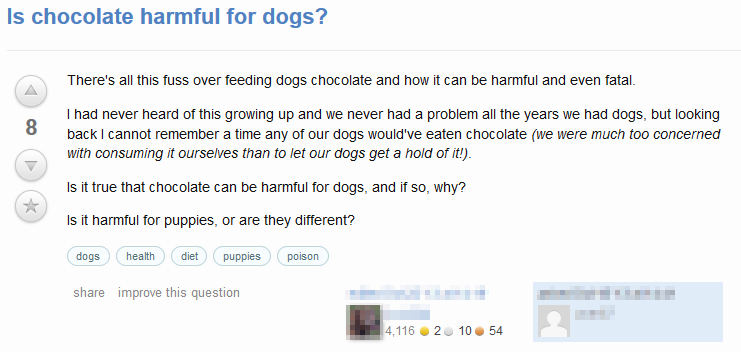
\includegraphics[width=100mm]{chap1/dog.PNG}
%\caption{The above example.}
%\end{figure}\label{gra:dog}

With over a billion active users and more than ten billion messages every day on Facebook \textsl{alone}\footnote{Taken from `A focus on Efficiency' by Facebook, Ericsson and Qualcomm 2013 (http://internet.org/efficiencypaper, September 16, 2013). Last accessed: March 10, 2014}, for example, there is a considerable amount of potentially inaccurate information being spread across social networks, and it would be desirable to be able to filter some of the wheat from the chaff.

This filtering of unsatisfactory content can take many different forms. Favourable content may `rise to the top' of a user's news feed in order of best to worst. Unfavourable content might be given some visual de-emphasis to indicate its lower quality, or may even be hidden from the user altogether. Users might be able to customize how strict this filtering is, or create whitelists and blacklists of people they trust and distrust respectively. In addition, users can be encouraged to improve their contributions to a community by gaining additional privileges or prestige for improving their reputation.

The rest of this report is structured as follows. In chapter two, a description is given of some reputation algorithms at a high level, and some case studies are examined of reputation systems currently in use online. In chapter three there will be an in-depth description of the producer-consumer model, collaboration events and constructing the collaboration graph, and using this graph to compute reputation. In chapter four there will be a description of the design and implementation of this project. In chapter five, there will be a description and justification of the data-sets and methodologies that were used, as well as a presentation of the results and findings. The final chapter presents the conclusions drawn in the course of this project, outlines criticisms of the project, and describes some possible future areas of research in the topic.

\chapter{Background Research}

% % %  CURRENTLY 7 / 10 PAGES

\section{Introduction}

The following chapter outlines the research undertaken into online reputation systems. Trust and reputation are explicitly defined, along with a brief explanation of their differences and why drawing a distinction between the two is important. Some research undertaken into user reputation algorithms that are currently in use across the web is presented. Finally, there are a number of case studies on sites that use a user reputation model, such as the Stack Exchange Network, eBay and Klout.


\section{Trust and reputation}

For the purposes of this project, \textsl{trust} is defined as a relationship between two parties. A trustor is an entity who places a certain amount of faith in the actions or knowledge of another entity (or the trustee). Trust is not a symmetric relationship, so while, for example, a student may trust a teacher's knowledge in their subject matter, the teacher will likely have less (or no) trust in their student's knowledge  (McNally, O'Mahony and Smyth 2013).

Trust can occur between numerous types of entities, such as between people or web-pages (Page, L., Brin S., Motwani, R., and Winograd, T. 1999). It is inherently a difficult property to quantify in any accurate way, and is why the need to draw a distinction between \textsl{trust} and \textsl{reputation} arises.

For the purposes of this paper, \textsl{reputation} is defined as a numeric measure of a user's \textsl{trustworthiness} according to some metric performed on their individual trust scores (McNally, O'Mahony and Smyth 2013).

There are a number of generic and ad-hoc implementation across the web. Examples of these are Google's PageRank algorithm for measuring a web-page's importance, Stack Exchange's system based on user activity, or eBay's implementation which uses user reviews to calculate reputation. Many of these implementations are bespoke systems, designed especially for their own domain. While these approaches may perform well, the development of a generic reputation algorithm which is applicable in many potential contexts would clearly beneficial. The development of such a generic reputation algorithm is the focus of this project.


\section{Reputation algorithms}

In the following section there is a discussion of a number of ways that reputation can be measured. In these techniques the term \textsl{producer} refers to a creator of content and \textsl{consumer} to the person who in turn receives that content. The word score refers to a number awarded to the \textsl{producers} for that content.

%\subsection{Weighted Sum}
%Description of Weighted Sum.

\subsection{TrustRank}

TrustRank is a link-analysis algorithm that evolved out of PageRank due to an abuse of the algorithm's weaknesses being exploited to create web-spam. The PageRank algorithm was developed by Page and Brin as they needed an approach to rank search results being presented to users by Google. It works simply by representing the web as a large graph, where web-pages are vertices, and links between them are directed edges between those vertices. PageRank assumes that the more incoming links a page has, the more popular and relevant it must be, and gives each vertex a PageRank score determined by the number of incoming edges it has and the scores of the vertices those edges originated from (Brin, Page 1998). Figure \ref{gra:pagerank} depicts a small network to which the PageRank has been applied. Larger vertex size is indicative of a higher PageRank score.

\begin{figure}[ht!]
\centering
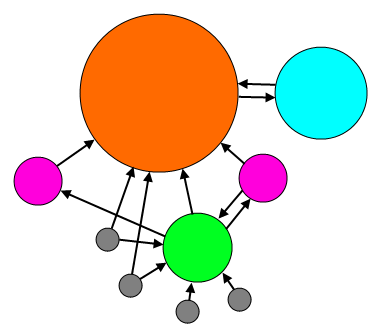
\includegraphics[width=80mm]{chap2/pagerank.png}
\caption{A visualisation of PageRank on a very small graph.}
\end{figure}\label{gra:pagerank}

The main vulnerability to the PageRank algorithm is that it can not differentiate between a legitimate incoming link and one manufactured to artificially inflate a page's score, which led to huge \textsl{link-farms}\footnote{http://www.nytimes.com/2011/02/13/business/13search.html} being created, where people bought and sold links to and from their sites to raise their rankings in search results.  To combat this, TrustRank creates a small set of \textsl{seed} pages which are manually verified by experts as being legitimate, non-spam web-pages. These seed pages are used to identify incoming links from other pages that are similarly `good', and this propagates through the graph as it is assumed a `good' page is unlikely to link to a `bad' page (Gyongyi et al. 2004).

\begin{figure}[ht!]
\centering
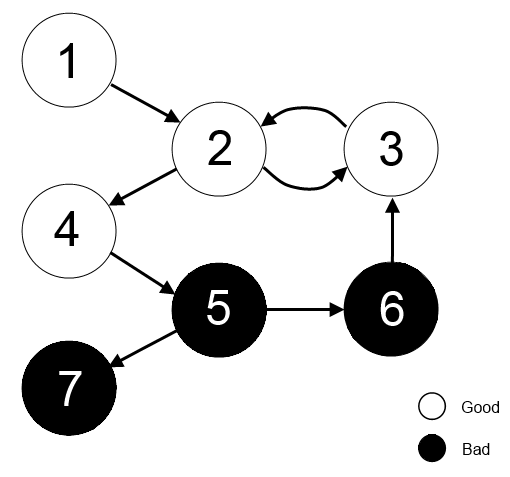
\includegraphics[width=60mm]{chap2/trustrank.png}
\caption{A graph of good and bad nodes, taken from Gyongyi et al. 2004.}
\end{figure}\label{gra:trustrank}

Pages can also be seeded negatively in the case that they are found to be `bad', and distrust can propagate through \textsl{outward} links from these pages, as bad pages are likely to link to other similarly bad pages. As figure \ref{gra:trustrank} demonstrates, TrustRank has some built in resistance to false-positives and negatives--cases where a `good' page links to a `bad' one and vice-versa can be accounted for due to nature of this positive and negative seeding. In this way the effect of manufactured links on page ranking results is significantly reduced.

\subsection{Trust-aware recommenders}

Traditionally, recommender systems use one of two approaches (or a hybrid of both) to produce a list of recommendations--content-based filtering, and collaborative filtering(Resnick et al. 1994; Balabanovic and Shoham 1997). 

Content-based filtering compares the properties of items to suggest similar ones to the end-user that they might like. This approach is often used to recommend things such as music and films. This can be less helpful in cases where a `more like this' form of recommendation tends to provide stale recommendations with little diversity or variety. Figure \ref{gra:amazon} demonstrates Amazon's recommendation system recommending batteries to a customer viewing a flash-light.

In collaborative filtering, the recommender system will instead compare the user's history against that of other users, and make recommendations based on shared viewing, purchase and feedback history (Breese et al. 1998). These recommendations, when relevant, are useful to both the user and the merchant. The user may be reminded to buy something they had forgotten, and the merchant makes another sale. This information can also be leveraged in other ways, for example a merchant may see that many items are bought together and bundle them at a small discount to encourage further sales.

\begin{figure}[ht!]
\centering
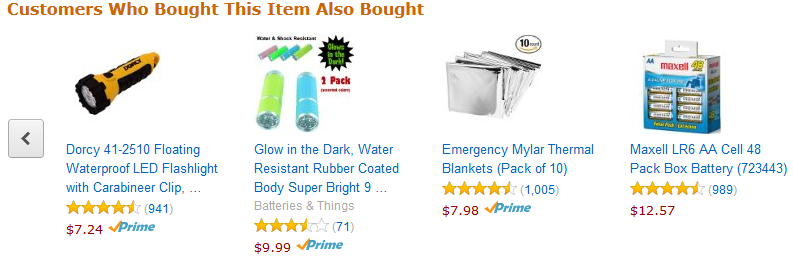
\includegraphics[width=140mm]{chap2/recommender.PNG}
\caption{Amazon recommending batteries, among other things, to a customer viewing a flash-light.}
\end{figure}\label{gra:amazon}

Like PageRank, however, these collaborative filtering recommender systems are vulnerable to manipulation. It is often a trivial matter for a person to fabricate a user and artificially create a viewing and feedback history tailored to draw users to their own products. To that end, there has been research into applying reputation to recommender systems (Massa and Avesani 2007; O'Mahony et al. 2004).

In his research, Massa proposes a reputation model whereby each user explicitly `rates' other users to create tailored trust statements. This system then aggregates all trust into a single trust network that represents all users' relationships. This trust network can be leveraged to filter out possibly untrustworthy recommendations from reaching the end user (Massa and Avesani 2007).

TODO: DESCRIBE JOHN O'DONOVAN'S WORK (O'Donovan and Smyth 2005).

%\subsection{Hubs and Authorities}
%Words go here.
\section{Case studies}

This section presents case studies for three bespoke user reputation models. The activity-based Stack Exchange model, eBay's user-feedback centric reputation model and Klout's social network influence score.

\subsection{Stack Exchange -- An activity based approach}

The Stack Exchange network\footnote{http://stackexchange.com/} is a collection of Question and Answer (Q\&A) communities, each focused on a specific field of expertise, with a site for everything from programming to bicycling and cooking. The network grew from the original Stack Overflow site, which focused on computer programming questions, and it is currently still the largest site in the network. As of the time of writing this report, the network consists of 114 Q\&A sites, almost 4.5 million users and over 8 million questions with 14.6 million answers.

\begin{figure}[ht!]
\centering
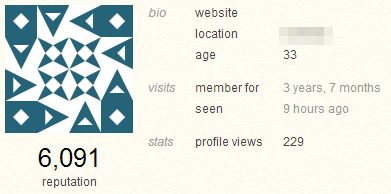
\includegraphics[width=100mm]{chap2/serep.png}
\caption{A cooking.stackexchange.com profile, showing reputation score.}
\end{figure}\label{gra:serep}

The Stack Exchange network uses a bespoke model of reputation. A user's reputation is calculated as a sum of points earned by contributing to the sites in various ways. Nearly every site activity, from asking and answering questions, to suggesting edits and flagging content for moderation can earn the user reputation points (see Figure \ref{tab:serep} for examples). This system is aimed more towards encouraging site activity than accurately evaluating a user's trust. A user can theoretically gain a considerable amount of reputation without actually demonstrating any domain knowledge.

\begin{minipage}{\linewidth}
\centering
\begin{tabular}{|l|l|}
\hline \textbf{Site activity} & \textbf{Reputation reward} \\ 
\hline Your question voted up & +5 \\ 
\hline Your answer voted up & +10 \\ 
\hline Your answer `accepted' as correct & +15 \\ 
\hline You `accept' an answer to your own question & +2 \\ 
\hline Your suggested edit accepted & +2 (up to a total of 1000) \\ 
\hline 
\end{tabular}\par
\captionof{table}{Stack Exchange reputation rewards.} \label{tab:serep}
\end{minipage}


Additionally, reputation can be lost for a number of reasons, ranging from abuse of the site, to low-quality submissions, although reputation never falls below 1. Moderation is largely performed by the community itself, as increasing reputation scores are rewarded with additional site privileges, ranging from moderation tools to access to chat-rooms.

A key limitation in addition to Stack Exchange's reputation scores reflecting activity rather than reputation, is that it is an ad-hoc system, tailored specifically to Stack Exchange's own needs and can not be easily applied to other domains

\subsection{eBay -- A feedback-based approach}

eBay Inc. is an online auction-house and market-place based entirely around user-to-user transactions. Originally founded in 1995, it has seen steady growth since, and has become the world's largest online marketplace, with over 112 million active users and \$175 billion USD worth of transactions facilitated by the site in 2012 alone\footnote{Taken from 'eBay Inc. Reports Strong Fourth Quarter and Full Year 2012 Results'. Available at: http://investor.ebayinc.com/releasedetail.cfm?ReleaseID=733959, last accessed March 10, 2014}.

With such a large volume of transactions passing through the site, evaluating trust is one of eBay's principle concerns. eBay calculates reputation using user feedback after transactions. For each positive transaction, the user's reputation score is increased by one point. If they receive neutral feedback, there is no change to their reputation, and if a transaction receives negative feedback, the user's reputation is decreased by one point.

In the event that there are multiple transactions between users in a single week, eBay aggregates the reputation points the user would have received. If this number is then positive, the reputation score is increased by one, if it is neutral, it does not change, and if it is negative, they lose one reputation point.

As a user's feedback score grows, they gain a coloured star next to their display name as a quick visual indicator of their reputation. Sellers who consistently gain lots of positive feedback and make frequent sales can also gain a `top-rated seller' badge that informs buyers that they consistently provide good service\footnote{Taken from `How feedback works'. Available at http://pages.ebay.co.uk/help/feedback/howitworks.html, last accessed 10th February 2014.}. An example of a user's feedback profile is given in Figure \ref{gra:ebay}.

Additionally, users can leave reviews with their feedback, where they may describe their interactions with the seller, the quality of the product, and the cost and speed of shipping.

\begin{figure}[ht!]
\centering
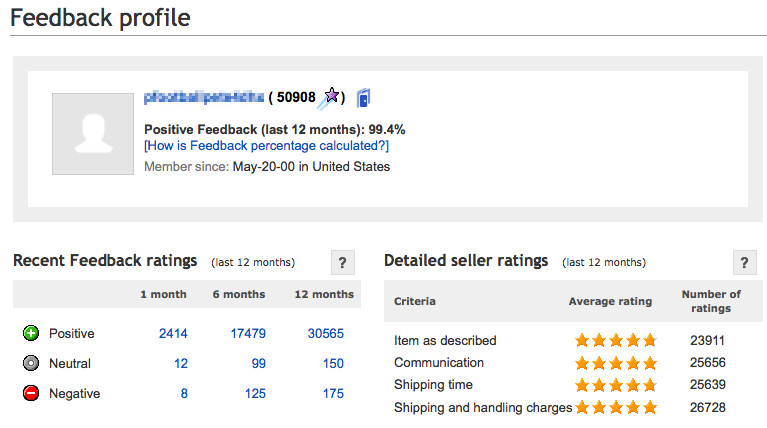
\includegraphics[width=140mm]{chap2/ebayfeedback.PNG}
\caption{An example of eBay feedback for one user.}
\end{figure}\label{gra:ebay}

This combination of easy to understand reputation score and collection of user reviews allows buyers to quickly find trustworthy sellers and decide from which of them they wish to conduct their business.

However, this approach has its limitations. As a whole, users receive very few negative feedback scores, and there is considerable evidence of a high degree of reciprocation in feedback scores (Resnick and Zeckhauser 2002).

\subsection{Klout -- A measure of influence}

Klout is an online service and mobile application that attempts to measure a user's \textsl{influence} across social networks. Launched in 2008, it uses analytics from eight different social media websites to evaluate its users' reputation scores, which is referred to as the \textsl{Klout Score}. This reputation score is an integer value bounded between 1 and 100, and becomes increasingly difficult to improve upon as it increases\footnote{http://klout.com/corp/about and http://klout.com/corp/score, last accessed accessed 10th March 2014}.

Among the metrics Klout uses to determine reputation are activity from Twitter, Facebook, the user's Wikipedia page (if one exists), Google+ and others. When a user produces content on these sites that gains `likes', generates discussion or is shared with others, Klout deems that this content generates \textsl{influence} to a lesser or greater degree, and so affects their Klout score.

\begin{figure}[ht!]
\centering
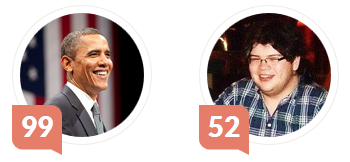
\includegraphics[width=80mm]{chap2/klout.png}
\caption{Barack Obama is considerably more influential than I am.}
\end{figure}\label{gra:klout}

Although Klout does not specify exactly how it calculates influence, there is evidence that the algorithms used on these \textsl{signals} or \textsl{collaboration events} are actually quite simple. In June, 2011, a Ph.D candidate in Montana State University, Sean Golliher, managed to calculate Klout's reputation score with an accuracy of 94\% simply by calculating a logarithm of the number of a user's followers and retweets\footnote{http://www.seangolliher.com/2011/uncategorized/how-i-reversed-engineered-klout-score-to-an-r2-094/}.

Besides being an ad-hoc system, the \textsl{Klout score} suffers the drawback that a high score is not necessarily indicative of knowledge or reputability in a specific context. A user may develop a high Klout score through a combination of celebrity status and regular use of social media.

\section{Conclusion}

This chapter has described some of the methods used to calculate reputation, and how different sites use reputation. It can be seen that many of these reputation models in the wild today are completely proprietary systems that require a lot of specific domain knowledge and are difficult to adapt for other uses. The main goal of this project is to demonstrate that a simplified, generic approach to reputation is an appropriate and viable alternative to engineering an ad-hoc reputation model. This generic approach shall be applicable to any domain in which there are producers and consumers of content.

\chapter{Creating a generic model of user reputation for the social web}
% % % 2 / 8 PAGES
This chapter provides an in-depth explanation of how to create a model of user representation for the social web that is generic and can be used in many contexts. The core concepts of this project such as the producer-consumer model of the social web, the collaboration event and collaboration graph, and exactly how to compute reputation are explained in depth.

\section{The producer-consumer model}

The producer consumer model is defined as a model of user relationships across an internet site in which there are trust interactions between \textsl{producers} and \textsl{consumers} of content. Trust interactions may be direct or indirect, and can be explicitly or implicitly defined (O'Donovan and Smyth 2005).

\begin{figure}[ht!]
\centering
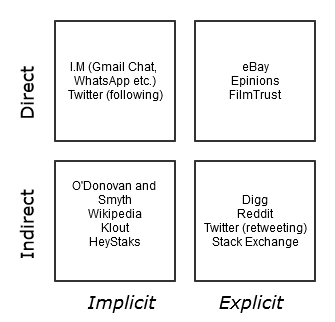
\includegraphics[width=90mm]{chap3/trusttypes.png}
\caption{Diagram demonstrating examples of direct, indirect, implicit and explicit trust interactions taken from McNally et al. 2013.}
\end{figure}\label{gra:trusttypes}

Direct trust interactions occur directly between two participants, that is to say that one user is rating another user in particular (more specifically a \textsl{consumer} is rating a \textsl{producer}), whether by following them on twitter or leaving a review on their eBay profile. Conversely, an indirect trust interaction does not occur directly between two users and may instead be a collective or community of \textsl{consumers} voting on a single \textsl{producer's} submission as opposed to voting on the \textsl{producer} themselves, for example people voting on an article submitted to Digg or Reddit, or multiple people retweeting a tweet. An explicit trust interaction is one in which the measure of trust being given is an explicit quantifiable signal, such as with a Reddit `up-vote' or an eBay review. Implicit trust interactions, then, are ones in which there is no explicit, easy to define signal that can be used to indicate the trust (McNally et al. 2013, refer to Figure \ref{gra:trusttypes} for examples).

The generic model of user reputation being investigated in the course of this project will be applicable to any producer-consumer interactions whether direct, indirect, explicit or implicit. Furthermore, this reputation model should be entirely generic, and applicable across a wide range of possible domains by identifying these trust interactions (McNally et al. 2013).

\section{The collaboration event}

Collaboration event is the name given to the flow of trust outlined above. Every 
collaboration event is a trust interaction between consumer and producer, and in many cases between consumer and multiple producers. For every collaboration event, the producers are awarded with some trust score, which may be positive, negative or neutral. When there is a single producer and consumer, the producer will receive the entirety of the trust score awarded by the consumer. In cases where there are multiple producers, the trust score will be divided among them, with each receiving a trust score corresponding to the perceived value of their contribution as compared to the other producers as seen in Figure \ref{gra:singlecollabevent}.

\begin{figure}[ht!]
\centering
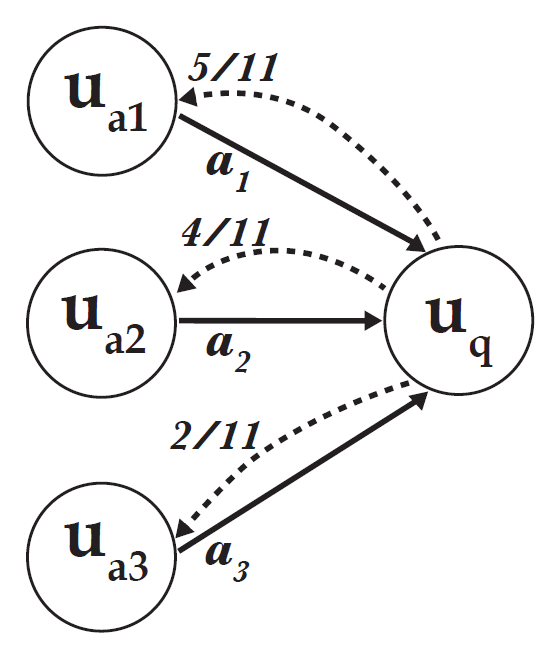
\includegraphics[width=40mm]{chap3/singlecollabevent.PNG}
\caption{A collaboration event with three producers and one consumer taken from McNally et al. 2013.}
\end{figure}\label{gra:singlecollabevent}

Identifying collaboration events varies in difficulty. In some instances, such as with an explicit trust interaction (see Figure \ref{gra:trusttypes}) it can be very simple, for example it may just be a unit of positive feedback on an eBay transaction. Other more implicit trust interactions may be more difficult to extract a collaboration event from. It is difficult to determine what some user activities and interactions may mean with regard to trust. A person's contribution to a Wikipedia page being edited may mean that their contribution was of poor quality, or it may simply mean that new information has since arisen that the editor has appended to the Wikipedia page.

To use Figure \ref{gra:singlecollabevent} as an example, a consumer on a Stack Exchange site, u$_{q}$, poses a question which receives three answers from the producers u$_{a1}$, u$_{a2}$ and u$_{a3}$. For their answers, these producers receive 5, 4 and 2 stack reputation (i.e. positive votes for their answers) respectively. As a total amount of 11 stack reputation is awarded for this collaboration event, u$_{a1}$ is rewarded $\frac{5}{11}$ of the reputation, u$_{a2}$ receives $\frac{4}{11}$ and u$_{a2}$ receives $\frac{2}{11}$ (McNally et al. 2013).

\section{Building the collaboration graph}

The collaboration events outlined above do not occur in isolation. Active users of these social networks may be involved in many collaboration events as both producer and consumer over time. The accumulation of these collaboration events can be represented by a directed weighted graph, with the users of the network as nodes in the graph, and the collaboration events between users represented by weighted directed edges between the users involved.

\begin{figure}[ht!]
\centering
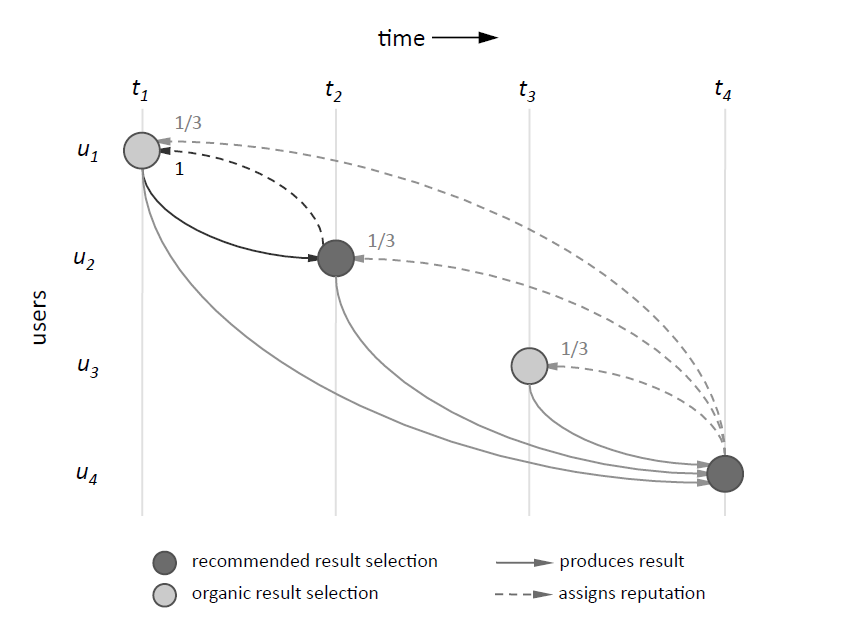
\includegraphics[width=130mm]{chap3/collabeventstime.PNG}
\caption{Demonstration of a series of collaboration events for social web-search recommendation tool HayStaks as a function of time (McNally et al. 2010).}
\end{figure}\label{gra:collabtime}

To build this graph, all of the collaboration events that make up this network must be examined in order over time. Figure \ref{gra:collabtime} demonstrates a small series of collaboration events as a function of time. At time t$_{2}$, the producer u$_{1}$ is assigned a unit of reputation by u$_{2}$ for their recommendation. At time t$_{4}$, producers u$_{1}$ u$_{2}$ and u$_{3}$ are each assigned a fraction of a reputation unit by u$_{4}$. As the number of collaboration events grows, so too does the graph which also becomes increasingly inter-linked, with the possibility for multiple edges in both directions between the same nodes as shown in Figure \ref{gra:collabgraph} where node $u_{c}$ is both a producer and consumer for nodes $u_{b}$ and $u_{d}$.

\begin{figure}[ht!]
\centering
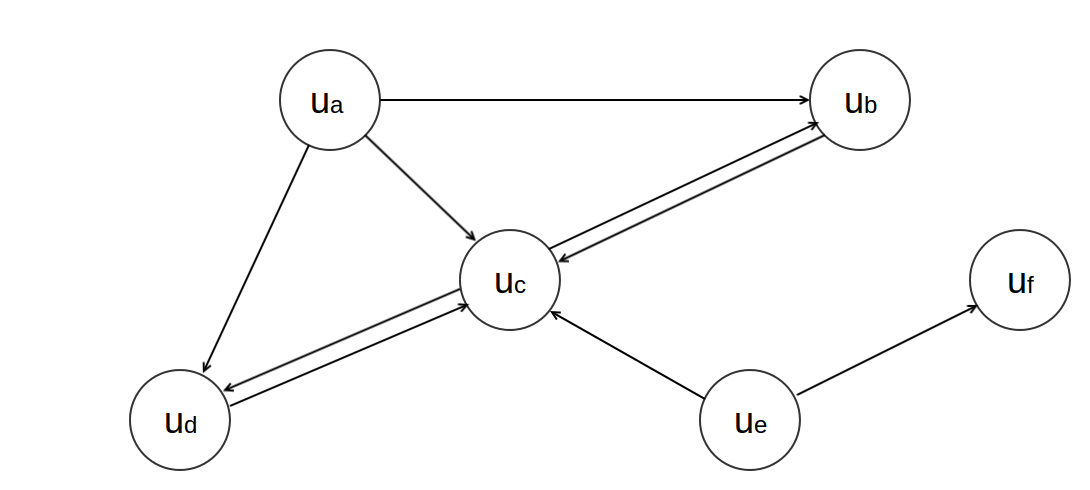
\includegraphics[width=100mm]{chap3/collabgraph.png}
\caption{Example of a collaboration graph with weights omitted.}
\end{figure}\label{gra:collabgraph}

\section{Computing reputation}

Once a collaboration graph has been constructed, it is then time to compute the reputation scores of the users in the graph. This project examined two algorithms from the literature (McNally et al. 2013) that can be leveraged to evaluate a reputation score for a user, Google's PageRank (Brin and Page 1998) and a simple in-degree Weighted Sum technique.

\subsection{Weighted Sum}

The Weighted Sum algorithm calculates the reputation score of a node by computing the sum of the weights of all incoming edges for that node. The formula for calculating reputation is as follows:
\[
rep(pi) = \sum_{e\in E_{pi}}^{} w_{e} 
\]
where $E_{pi}$ is the set of incoming edges for the producer $p$, $_{e}$ is the current incoming edge and $w_{e}$ is the weight of $_{e}$. This Weighted Sum model encourages users to gain reputation by becoming producers of content across many questions and may cause an increase in the number of producers, for example users on the Stack Exchange network may feel more inclined to provide answers for questions. This model may also lead to less repetition of information as a user is less likely to receive as much reputation for simply repeating an answer that has already been given, instead producers are encouraged to produce their own unique content (McNally et al. 2013).

%This algorithm has the benefit of being generic. It can apply to a wide range of contexts. For example with the social media platform Twitter, `retweets' can fit into our collaboration event model and the Weighted Sum can be calculated as a ratio of the consumers' retweets over time. If a producer's tweet is retweeted by five consumer, and between them those five consumers have retweeted a total of thirty-five tweets, the producer may gain a reputation score of $\frac{5}{35}$ for the production of that content.

\subsection{PageRank}

PageRank is perhaps one of the most well-known link-analysis algorithms in use today. Originall developed by Sergey Brin and Larry Page at Google (Brin and Page 1998), it works by making the assumption that important pages in the web (or nodes in a graph) are also the ones most fequently linked to, and that the more important a page or node is, the more weight its own links to other pages should carry (see Figure \ref{gra:pagerank} for a visual example). This insight into the nature of the structure of hyper-linked web-pages allowed them to create the PageRank algorithm to sort results for the Google search engine.

The PageRank algorithm is slightly more complex than the Weighted Sum. The PageRank score for each user $p_{i}$ is computed as thus:
\[
rep(p_{i}) = \frac{1 - d}{N} + d \sum_{p_{j} \in M(p_{i})} \frac{PR(p_{j})}{|L(p_{j})|}
\]
where $d$ is a damping factor, $N$ is the number of users, $M(p_{i})$ is the set of in-links from consumers to the producer $p_{i}$ and $L(p_{j})$ is the set of out-links from $p_{j}$ (i.e. the users from which $p_{j}$ has consumed content). In the context of the Stack Exchange network, the PageRank score for a given user can be thought of as the likelihood that a randomly selected `good' answer will have been given by that user (McNally et al 2013).

\section{Predicting quality answers using reputation}

Placeholder until answer prediction is finished. Describe the methodology of answer prediction (the 80/20 fitting/testing split).

\section{Conclusion}

In conclusion, it has been demonstrated that it is possible to create a model of user reputation in a generic fashion when there are consumers and producers of content. With a little thought it is possible define appropriate collaboration events with which a collaboration graph can be built, which can then be leveraged to compute reputation for users using a variety of algorithms.. 

\chapter{Design \& Implementation}

% % % 5/6 PAGES

\section{Project structure}

Throughout this project, every attempt has been made to ensure the code written is as concise, clear and efficient as possible. What follows is an attempt to give a brief explanation of the structure of the project and a description of what each class does where appropriate. 

The main, root class named `FYP' begins by finding the user's home directory, and then spawning the `ParserLauncher' class with the sub-directory of home named `stack' as a parameter. This ParserLauncher checks the `stack' directory for any sub-directories. 

For each sub-directory found, it is assumed that this directory will contain the input files Users.xml and Posts.xml that need to be parsed, and will launch the appropriate parsers. Once the files have been successfully parsed, the `ParserLauncher' then creates a `GraphBuilder' class. Finally, this `GraphBuilder' class generates the Gephi graphs that will be used later on to computer reputation scores.

A UML class diagram of this project structure can be seen in figure \ref{fig:classdiagram}.
\newpage
\begin{figure}[ht!]
\centering
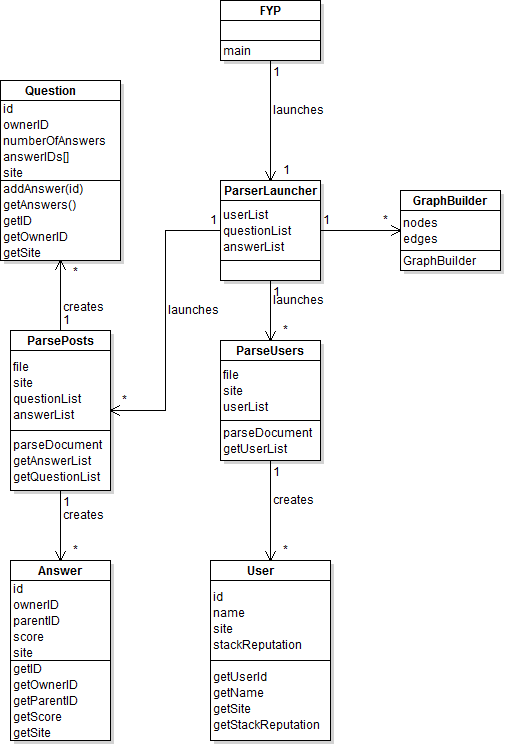
\includegraphics[width=140mm]{chap4/classdiagram.png}
\caption{Class diagram of the overall project structure.}
\end{figure}\label{fig:classdiagram}

\newpage
\section{Development tools}

A number tools were used throughout this project. The majority of the code was written in Java.\footnote{Oracle's Java 1.7 on Windows machines and OpenJDK 7 on Unix.} Apache's Maven was used for dependency management via the m2e plugin bundled with the Eclipse IDE. Initially a PostgreSQL\footnote{http://www.postgresql.org/} database was used for persistent storage of data, and the Flyway and JDBI\footnote{http://flywaydb.org/ and http://jdbi.org/} Java libraries were used for handling database migrations and executing queries respectively, however the database was abandoned for an in-memory model instead when it became clear the data-sets were suitably small.

All code and the contents of this report were kept under version control using git, with a remote on GitHub.com\footnote{https://github.com/JackBracken/FYP} as a backup. In addition, Gephi\footnote{https://gephi.org/} was used to construct the graph and Matlab was used to perform analysis on the results.

\section{Obtaining the data}

The Stack Exchange network publishes quarterly dumps of all user-generated content on the Internet Archive.\footnote{http://blog.stackoverflow.com/2014/01/stack-exchange-cc-data-now-hosted-by-the-internet-archive/} Data is sanitised to remove private user information, then published in XML format that closely mirrors the tables in a Stack Exchange database, with each XML object corresponding to a row in a conventional relational database. Files can be downloaded directly, or through the BitTorrent protocol (which is encouraged) which also allows a user to seed\footnote{BitTorrent is a peer-to-peer file-sharing protocol. `Seeding' is its term for remaining connected to the network to continue uploading whatever file(s) you have downloaded for the good of the network.} the data for a while if they wish to contribute back in some way.

Once the data has been downloaded, it must be removed from the archives using the 7zip protocol, and kept somewhere safe. For this project I created a directory named stack in my `HOME' directory. Each site's data files should be kept in their own sub-directory--my implementation assumes that these sub-directories share the same name as the site they originated from. Of these XML files, the Users and Posts files must be left as is, the others may be removed or left alone--they will be ignored regardless. 

The Users and Posts files are then parsed, and the data is stored in one of three HashMaps for users, questions and answers each, with their unique ID numbers used as keys for easy retrieval. The Key-Value access of a HashMap allows convenient and fast lookup of objects by their unique ID number if it is used as a key as retrieving an Object by its key is an O(1) average-case operation.

\subsection{Processing users}

Each User artefact in the Users file contains data corresponding to their unique identifying number, user name, their reputation on this Stack Exchange network and so on. Much of the data provided is extraneous for the purposes of this project and is ignored. When the Users file is parsed, the only data taken directly from it is the user's ID, their user-name and reputation score on that site.

\subsection{Processing posts}

As with the Users file, the Posts file contains a large amount of information that is unneeded for this project, such as the number of views a post has and its edit history. For the purposes of this project the only data that is parsed is the post's unique ID, the ID of the author of the post, the post type, the ID of the parent post (if this is an answer) or the number of responses this post has received (if it is a question), and the post's Stack Exchange score.

As we are not told directly whether a post is a question, answer, or something else, we must manually infer this ourselves from the PostTypeId field. Each integer from 1 - 8 corresponds to a post type. Since we are only concerned with questions and answers, any post which does not have a PostTypeId of 1 or 2 is ignored. See Table \ref{tab:posttypes} for a full list of post type IDs.

\begin{minipage}{\linewidth}
\centering
\begin{tabular}{|l|l|}
\hline \textbf{Id} & \textbf{Value} \\ 
\hline 1 & Question \\ 
\hline 2 & Answer \\ 
\hline 3 & Wiki \\ 
\hline 4 & TagWikiExcerpt \\ 
\hline 5 & TagWiki \\ 
\hline 6 & ModeratorNomination \\ 
\hline 7 & WikiPlaceholder \\ 
\hline 8 & PrivilegeWiki \\
\hline 
\end{tabular}\par
\captionof{table}{Post type IDs and their meanings.} \label{tab:posttypes}
\end{minipage}

\subsection{Building the graph}

Once the user, question and answer data has been successfully parsed, it is time to create the graph of collaboration events. For this project, the Gephi tool-kit\footnote{The tool-kit is a Java library which allows developers to create and interact with Gephi graphs through its API: https://gephi.org/toolkit/} is used to create a graph file which can be interacted with using the Gephi application.

To create this file, first the graph is populated with nodes. This is a simple matter of iterating through the HashMap of users, creating a new node for each user, and appending them to the graph. For the node labels, the user's Stack Exchange reputation score and user-name separated by a comma are used, for easier retrieval later, as Gephi does not provide a facility to insert extra meta-data in nodes. The graph is then populated with the edges that correspond to collaboration events. Every answer is iterated over and used to to draw the edges between the answer and its parent question, along with the edge weight, which is the score that the answer received. 

Once the nodes and edges have been successfully appended to the graph, creation of the graph file is accomplished using the tool-kit's ExportController class. This class can create either a PDF document with a visualization of the graph or a Gephi graph file with the .gexf extension. Which type of file is created simply depends on the file extension used when writing. The implementation of this project creates a separate graph file for each network examined.

\begin{program}
\begin{verbatim}
ExportController ec = Lookup.getDefault().lookup(ExportController.class);
try {
    ec.exportFile(new File(siteName + ".gexf"));
} catch (IOException e) {
    e.printStackTrace();
}
\end{verbatim}
\caption{Writing the graph to file.}
\end{program}

\section{Computing reputation scores}

Gephi makes it a simple matter to computer the In-degree Weighted Sum and PageRank scores for the nodes in our graph, among other things. Open the generated graph file in Gephi. In the right-hand pane of the overview tab, there is a statistics view, which can be used to compute statistical data for the nodes and edges of the graph by clicking the corresponding `run' button. Once this is done, a report view is displayed which can be ignored.

%\begin{figure}[ht!]
%\centering
%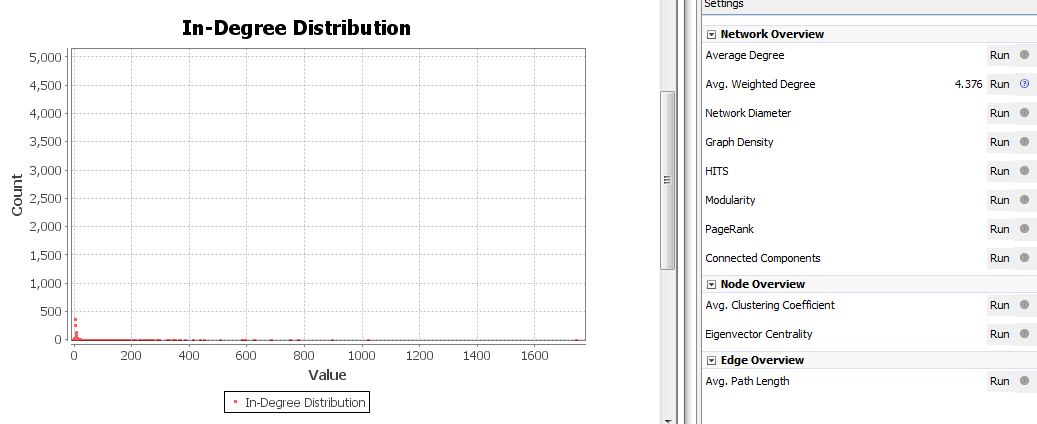
\includegraphics[width=80mm]{chap4/gephistats.png}
%\caption{Gephi stats pane and report view.}
%\end{figure}\label{gra:gephistats}

\begin{figure}[ht!]
\centering
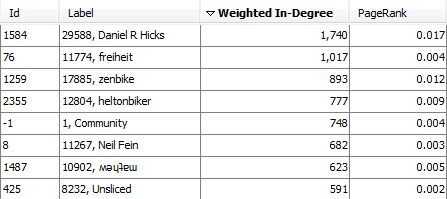
\includegraphics[width=100mm]{chap4/gephidata.PNG}
\caption{Gephi data-lab showing users on the bicycles stack exchange network sorted by Weighted Sum score.}
\end{figure}\label{gra:gephidata}

Once the Weighted Sum and PageRank values have been computed, they are inserted into the `Data Laboratory' view. From this view it is possible to interact with the data in a number of ways, from searching for specific nodes, adding, deleting and duplicating nodes or edges, sorting by property (see Figure \ref{gra:gephidata}), and changing the properties of nodes. It is also possible to export this data to a comma-separated-value file for later analysis.

\section{Predicting correct answers}

Placeholder until answer prediction completed

\chapter{Testing \& Evaluation}



\section{The data-sets}

For the purposes of this project, three different data-sets were selected 

\begin{minipage}{\linewidth}
\centering
\begin{tabular}{|l|r|r|r|}
\hline
\multirow{2}{*}~ & \multicolumn{3}{c|}{\textbf{Dataset}} \\
\cline{2-4}
~ 					& Bicycles & Cooking & Electronics \\ \hline\hline
\# Users 			&  8,009 &  15,802 &  25,335 \\ \hline
\# Questions asked 	&  4,023 &   9,037 &  24,404 \\ \hline
\# Answers given 	& 12,196 &  24,679 &  49,006 \\ \hline
\# Answers on votes & 62,974 & 130,446 & 210,694 \\ \hline
\end{tabular}\par
\captionof{table}{Statistics for the three Stack Exchange sites used in the course of this project--the bicycles, cooking and electronics sites.} \label{tab:corrresults}
\end{minipage}

\section{Methodology}

\section{Analysis}

%*class(es) for analysis - e.g. to compute correlations between rep model scores and to evaluate accuracy of predicted answers
Once the csv files were created, I then opened them up using spreadsheet software\footnote{LibreOffice Calc in my case, but any will suffice.} to extract the data for Matlab. Because the Weighted Sum score as a model of reputation is the `main' focus of this project, I sorted the data by the Weighted Sum column in descending order. Due to the fact that a large number of users never deign to answer any questions, and our reputation scores are based off of the Producer-Consumer model, we end up with a large number of users with no Weighted Sum score, so we discard these.



Now that we have the data, it is time to analyse it with Matlab. Column vectors were created for the SE, WS and PR scores, the scores are all normalised to be between 0 and 1, and the results are then plotted on a histogram to be compared with previous research and ensure the results seem to be within bounds. Histograms were created for each algorithm before being super-imposed over each other using an image manipulation program, the results of which can be seen in \ref{fig:histogram}.

%\begin{program}
%\begin{verbatim}
%se = [29588 11774 17885 12804 11267]'
%normalised_se = se/max(se)
%hist(normalised_se)
%\end{verbatim}
%\caption{Normalising a vector and plotting a histogram of its values.}
%\end{program}

After the histograms of normalised user score vs. number of users were generated, it was then time to analyse the correlation between reputation algorithm scores. To do so, for each site being evaluated, three rounds of analysis were performed. One round on the top 10 users by WS score, a second by the top 50 users by WS score, and finally once for all users with computable WS scores. For each round of analysis, a column vector was created for each of the SE, WS and PR scores. The correlation was then found between each permutation of reputation score (i.e., between SE and WS, SE and PR and between WS and PR), and both the Pearson and Spearman correlation scores were computed and recorded in each case.

%\begin{program}
%\begin{verbatim}
%se = [29588 11774 17885 12804 11267]'
%ws = [1740 1017 893 777 682]'
%corr(se, ws, 'type', 'Pearson')
%ans =
%    0.9219
%corr(se, ws, 'type', 'Spearman')
%ans =
%    0.7000
%\end{verbatim}
%\caption{Creating column vectors with SE and WS scores, then computing Pearson and Spearman correlation with results shown.}
%\end{program}

The results of this analysis can be found in table \ref{tab:corrresults} and are discussed at length there.

\section{Evaluating performance}

%\begin{figure}[ht!]
%\centering
%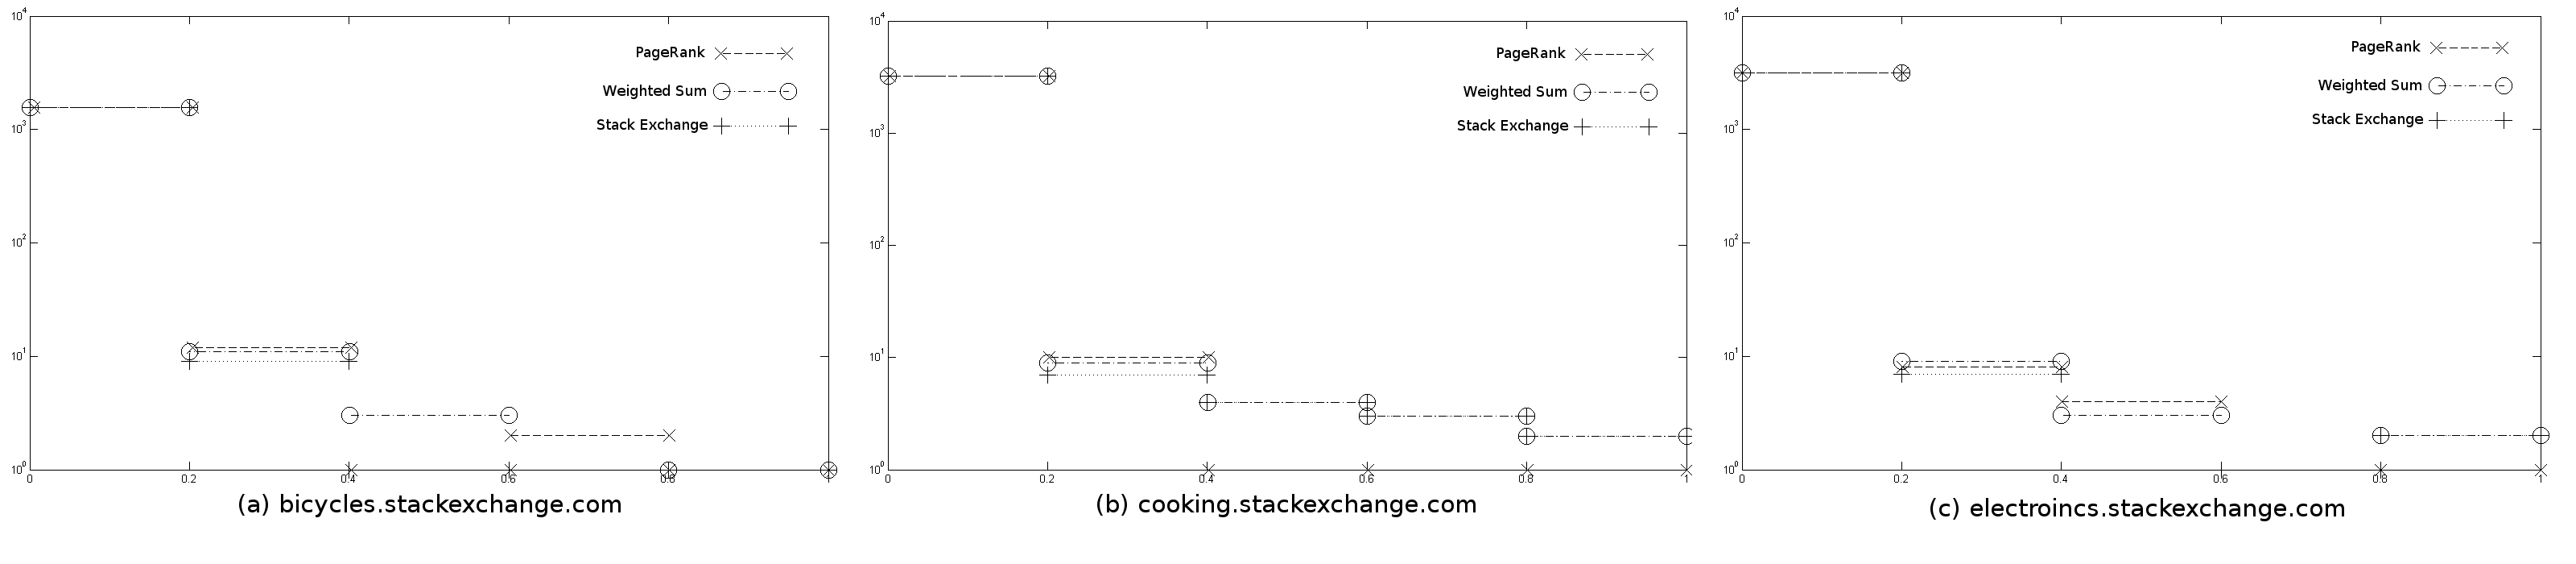
\includegraphics[width=160mm]{chap3/histograms.png}
%\caption{Distribution of reputation scores across different sites and algorithms.}
%\end{figure}

Remake this figure zoomed in more with less nodes and add labels (maybe make node size representative of rep)
\begin{figure}[ht!]
\centering
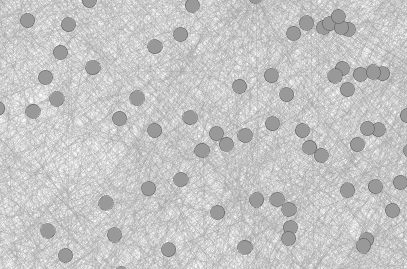
\includegraphics[width=100mm]{chap4/gephigraph.PNG}
\caption{A close-up view of the graph created from the bicycles network data.}
\end{figure}\label{gra:network}

\begin{figure}[ht!]
\centering
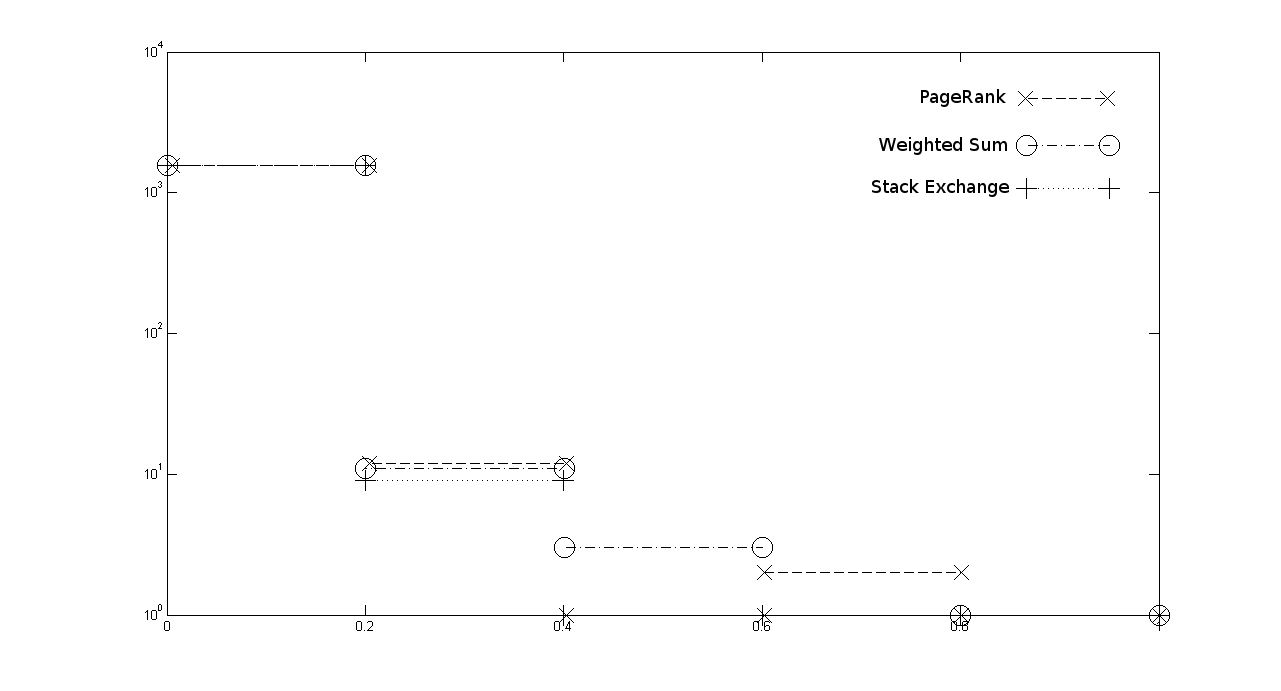
\includegraphics[width=120mm]{chap3/bicycles_hist.png}
\caption{Distribution of reputation scores across the Bicycles SE network.}\label{fig:histogram}
\end{figure}\label{gra:bicyclehist}

\begin{figure}[ht!]
\centering
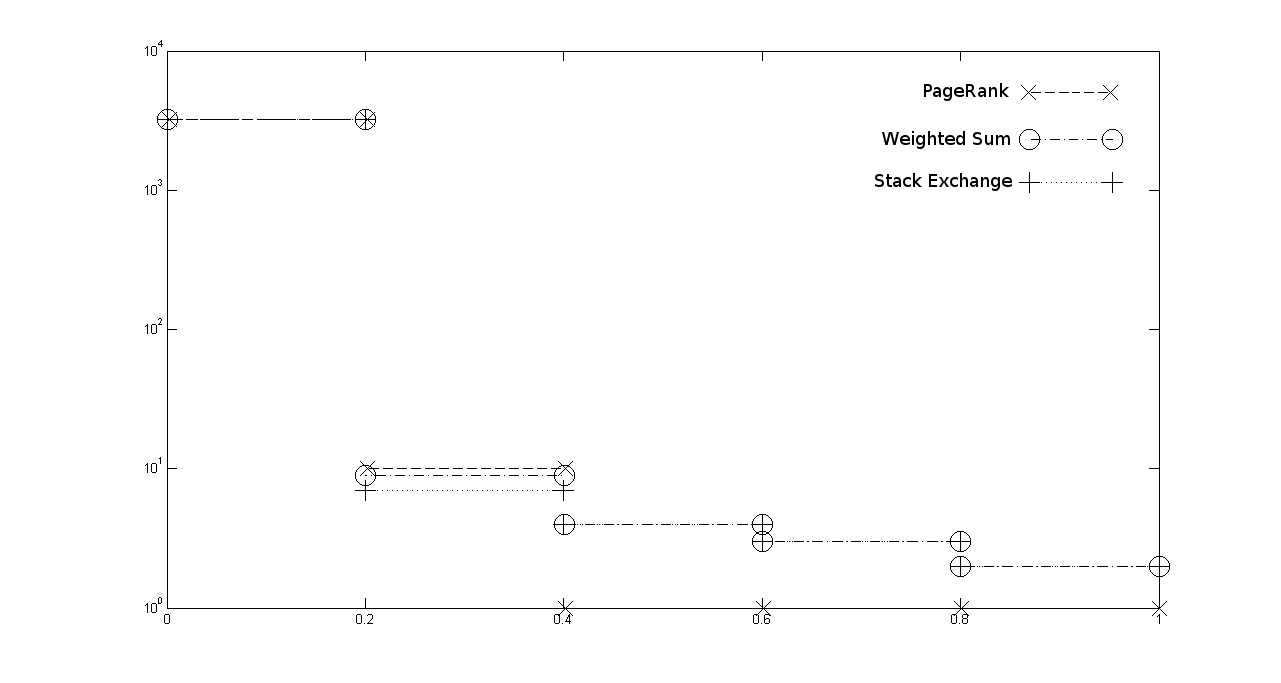
\includegraphics[width=120mm]{chap3/cooking_hist.png}
\caption{Distribution of reputation scores across the Seasoned Advice SE network.}
\end{figure}\label{gra:cookinghist}

\begin{figure}[ht!]
\centering
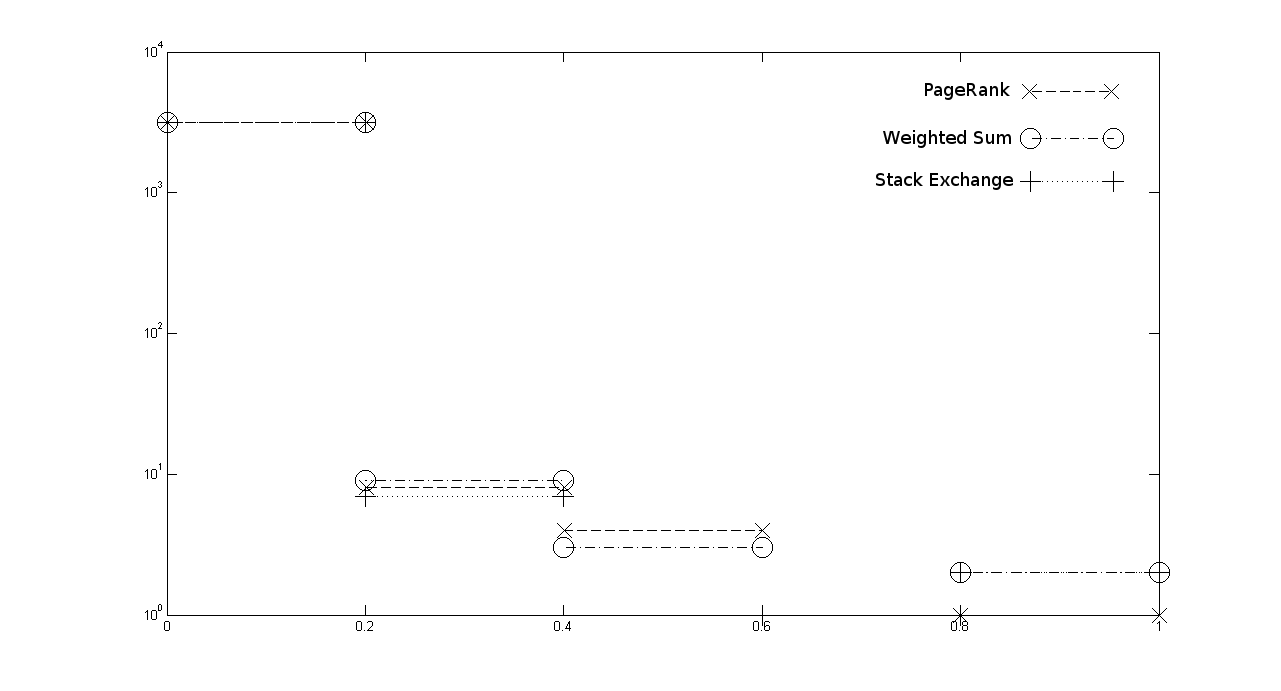
\includegraphics[width=120mm]{chap3/electronics_hist.png}
\caption{Distribution of reputation scores across the Electronics SE network.}
\end{figure}\label{gra:electronicshist}

Long-tailed distribution in histograms. Talk about scores being normalised between 0 and 1. Describe the histograms

\section{Correlation analysis}

Discuss the correlation results. Low Spearman rank means results ordered very differently, think about why and explain.

% Table of results for correlation analysis
\begin{minipage}{\linewidth}
\centering
\begin{tabular}{|l|l||l|l|l||l|l|l|}
\hline
\textbf{Site} & \textbf{Users} & \multicolumn{3}{l||}{\textbf{Pearson}} & \multicolumn{3}{l|}{\textbf{Spearman}} \\ \hline
\multicolumn{2}{|l||}{\textbf{Correlations between}} & \textbf{SE/WS} & \textbf{SE/PR} & \textbf{WS/PR} & \textbf{SE/WS} & \textbf{SE/PR} & \textbf{WS/PR} \\
\hline
~ 					& Top 10 & 0.9523 & 0.8225 & 0.7222 & 0.9515 & 0.5636 & 0.4182 \\      
\textbf{Bicycles}	& Top 50 & 0.9791 & 0.8846 & 0.8501 & 0.9520 & 0.8023 & 0.8082 \\
~ 					& All    & 0.9838 & 0.8966 & 0.8785 & 0.8237 & 0.5140 & 0.5434 \\
\hline
~           		& Top 10 & 0.9656 & 0.6547 & 0.5103 & 0.9394 & 0.3455 & 0.4545 \\
\textbf{Cooking}    & Top 50 & 0.9901 & 0.7855 & 0.7536 & 0.9501 & 0.6267 & 0.6700 \\
~          			& All    & 0.9920 & 0.8800 & 0.8690 & 0.8255 & 0.5130 & 0.5254 \\
\hline
~           		& Top 10 & 0.9881 & 0.7840 & 0.8204 & 0.9515 & 0.7212 & 0.8545 \\
\textbf{Electronics}& Top 50 & 0.9922 & 0.8716 & 0.8948 & 0.9669 & 0.6926 & 0.7247 \\
~           		& All    & 0.9893 & 0.9116 & 0.9276 & 0.7649 & 0.5204 & 0.5703 \\
\hline
\end{tabular}\par
\captionof{table}{Stack Exchange reputation rewards.} \label{tab:corrresults}
\end{minipage}

\section{Coverage}

\begin{minipage}{\linewidth}
\centering
\begin{tabular}{|l|l|}
\hline \textbf{Site} & \textbf{\% users with WS score} \\ 
\hline Bicycles & 19.60\% \\ 
\hline Cooking & 20.61\% \\ 
\hline Electronics & 12.59\% \\ 
\hline 
\end{tabular}\par
\captionof{table}{Coverage of users with computable WS scores.} \label{tab:coverage}
\end{minipage}

Charts detailing coverage (include PageRank)

\section{Predicting the answers to questions}

Placeholder until answer prediction finished. Train on first 80\% of questions (fitting), compute rep scores. Final 20\% attempt to predict the correct answers 

\chapter{Conclusions \& Future Work}

Placeholder

\section{Fulfilment of project goals}

Address the stated project goals, which ones were attempted, and success in completing them

\section{Learning outcome}

Outline learning outcomes throughout the course of this project

\section{Failings}

What didn't work? What could have been done better? Criticisms of approach to the project.

\section{Future work}



%%%% ADD YOUR BIBLIOGRAPHY HERE
\newpage
\raggedright
\textbf{McNally, K., O'Mahony, M.P., and Smyth, B. 2013} -- ``A Model of Collaboration-based Reputation for the Social Web.'' FIX REFERENCE
\linebreak
\linebreak
\textbf{Cheng, R., and Vassileva, J. 2005} -- ``Reward Mechanism for Sustainable Online Learning Community.'' Proceedings of the 2005 conference on Artificial Intelligence in Education. IOS Press.
\linebreak
\linebreak
\textbf{Page, L., Brin S., Motwani, R., and Winograd, T. 1999} -- ``The PageRank citation ranking: Bringing order to the Web.''
\linebreak
\linebreak
\textbf{Mui, L. 2002} -- ``A Computational Model of Trust and Reputation.'' Agents, Evolutionary Games, and Social Networks
\linebreak
\linebreak
\textbf{Resnick, P., Zeckhauser, R.} -- ``Trust Among Strangers in Internet Transactions: Empirical Analysis of eBay's Reputation System.'' Advances in Applied Microeconomics 11, 2002, p127-157
\linebreak
\linebreak
\textbf{Gyongyi, Z., Garcia-Molina, H., Pedersen, J.} -- ``Combating Web Spam with TrustRank.'' Proceedings of the Thirtieth International Conference on Very Large Data Bases (2004), Volume 30, p576-587
\linebreak
\linebreak
%\textbf{O'Donovan, J., Smyth, B.} -- ``Trust in Recommender Systems.'' In IUI 2005: Proceedings of the Tenth International Conference on Intelligent User Interfaces, p167-174
%\linebreak
%\linebreak
\textbf{Massa, P., Avesani, P. 2007} -- ``Trust-Aware Recommender Systems.'' In Proceedings of the 2007 ACM conference on Recommender systems. ACM. p17-24
\linebreak
\linebreak
\textbf{Breese, J.S., Heckerman, D., Kadie, C.} -- ``Empirical Analysis of Predictive Algorithms for Collaborative Filtering.'' In Proceedings of the Fourteenth Conference on Uncertainty in Artificial Intelligence, Morgan Kaufmann Publishers Inc., May 1998, p43-52.
\linebreak
\linebreak
\textbf{Brin, S., Page, L.} -- ``The anatomy of a large-scale hypertextual Web search engine.'' Computer networks and ISDN systems 30.1, 1998, p107-117.
\linebreak
\linebreak
\textbf{Hoorens, V.} -- ``Self-enhancement and Superiority Biases in Social Comparison.'' The European Review of Social Psychology (1993), Volume 4, Issue 1 p113-139
\linebreak
\linebreak
\textbf{Jøsang, A., Ismail, B., Boyd, C.} -- ``A survey of trust and reputation systems for online service provision.'' Decision Support Systems, Volume 43, Issue 2, March 2007, p618–644
\linebreak
\linebreak
\textbf{McNally, K., O'Mahony, M., Coyle, M., Briggs, P., Smyth, B.} -- ``A Case Study of Collaboration and Reputation in Social Web Search.'' In ACM Transactions on Intelligent Systems and Technology, Volume 9, No. 4, Article 39, March 2010, p39-69
\linebreak
\linebreak
\textbf{Resnick, P., Iacovou, N., Suchak, M., Bergstrom, P., Riedl, J.} -- ``Grouplens: An Open Architecture for Collaborative Filtering of Netnews.'' In Proceedings of ACM CSCW’94 Conference on Computer-Supported Cooperative Work, Sharing Information and Creating Meaning, 1994, p175–186
\linebreak
\linebreak
\textbf{Balabanovic, M., Shoham, Y.} -- ``Fab: Content–based, Collaborative Recommendation.'' Communications of the ACM , Vol. 40, No. 3, ACM Press, March, 1997, p66–72
\linebreak
\linebreak
\textbf{O’Mahony, M., Hurley, N., Kushmerick, N., Silvestre, G.} -- ``Collaborative Recommendation: A Robustness Analysis.'' ACM Transactions on Internet Technology (TOIT), Special Issue on Machine Learning for the Internet, Vol. 4, No. 4, ACM Press, November, 2004, p344–377
\linebreak
\linebreak
\textbf{O'Donovan, J., Smyth, B.} -- ``Trust in Recommender Systems''. In Proceedings of the 10th International Conference on Intelligent User Interfaces (IUI '05). ACM, New York, NY, USA, 2005, p167-174

%\textbf{McNally, K., O'Mahony, M., Smyth, B.} -- ``A Comparative Study of Collaboration-based Reputation Models for Social Recommender Systems''

%\begin{thebibliography}{99}


%\end{thebibliography}
\label{endpage}

\end{document}

\end{article}
